
\documentclass[11pt]{article} 

\usepackage[utf8]{inputenc} 
\usepackage{geometry} 
\geometry{a4paper} 

\vspace{2cm}
\setlength{\parindent}{0cm}
\usepackage{graphicx,wrapfig,placeins}

\title{Interactive Graphics}
\author{Chichi Francesco, Jary Pomponi}

\begin{document}
\maketitle
\graphicspath{{img/}}
\section{Introduction}
	The project developed from us is a local multi player game (1-4 players), inspired to the film \textit{Tron}.\\
	The goal of each player is to eliminate all the other players, and to do so, he have to traps them in some walls.
	When a player bump a wall or another player, he dies. At this point, the animation of the death start, and when it's ended, the ship and the relative walls disappear from the map.
\section{List of all the libraries, tools and models used in the project but	not developed by the team}
\begin{itemize}
	\item \textbf{Three.js:}
		Three.js is a cross-browser JavaScript library/API used to create and display animated 3D computer graphics in a web browser exploiting the power of WebGL in an high level mode.
	\item \textbf{OrbitControls.js:}
		We used OrbitControls to allow the user to move the camera in the space.
	\item \textbf{Detector.js:}
		Detector is necessary to verify if the user's browser support \textit{WebGL}.
	\item \textbf{stats.min.js:}
		stats.min is used to show the FPS, frame per second, or the MS, the millisecond used for each render.
		
\end{itemize}
\newpage
\section{Description of all the technical aspects of the project}
\subsection{Ship}
	

	\begin{wrapfigure}{r}{0pt}
		\centering
		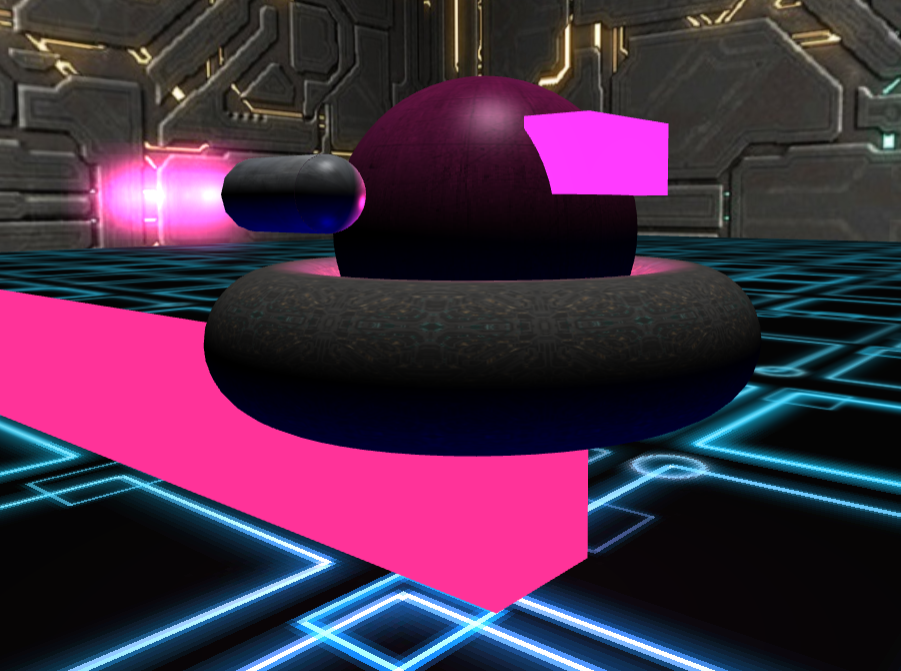
\includegraphics[width=0.4\linewidth]{ship}
		\caption{This is the character of a player that choosen the pink colour.}
		\label{fig:ship}
	\end{wrapfigure}

	
	Each player has a ship of the choosen colour, which one is a three.js Group, composed by a \textbf{cabin} (fig. 2), a clock wise rotating \textbf{ring} (fig. 3) and two \textbf{motors} (fig. 4).\\
	
	The cabin is also a Group of element coloured with the player's colour, composed by a glass and a cockpit with a pointlight inside.
	The cockpit is a sphere covered with a metallic texture, the glass is a parallelepiped made by a \textit{MeshToonMaterial}, that is illuminated by the cockpit's light.\\
	
	Each motor is another independent Group, composed by a cylinder, an hemisphere on the top and another hemisphere with an hole, that represent the exhaust pipe, each one is covered with the metallic texture of the cabin.
	Furthermore, at the end of the exhaust pipe, there are 50 particles of the colour of the player. The wake's length where this particles are distributed is choosen stochastically: with a probability of 80\%, the wake's length is equal to 40, with 10\% is 0 or 10.\\
	
	Finally, there is a rotating ring, that is a torus coloured with the same texture of the torus which rotates around the map.
	
	\begin{figure}
		\centering
		\begin{minipage}[b]{0.25\linewidth}
			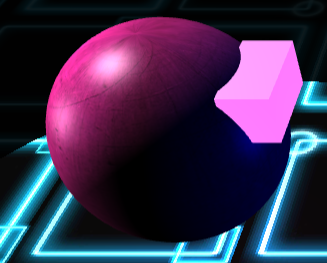
\includegraphics[width=\linewidth]{cabin}
			\caption{The cabin of the ship.}
			\label{fig:cabin}
		\end{minipage}
		\begin{minipage}[b]{0.276\linewidth}
			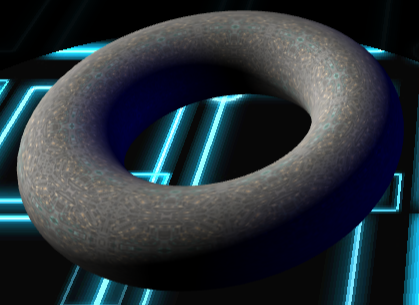
\includegraphics[width=\linewidth]{toro}
			\caption{The rotating torus.}
			\label{fig:toro}
		\end{minipage}
		\begin{minipage}[b]{0.6\linewidth}
			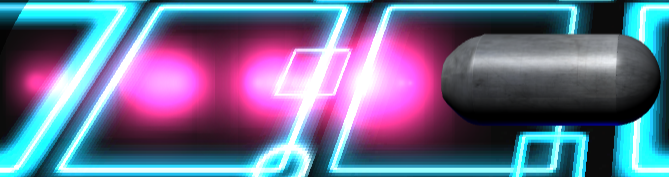
\includegraphics[width=\linewidth]{motor}
			\caption{A motor with the particles.}
			\label{fig:motor}
		\end{minipage}
	\end{figure}

\FloatBarrier



\subsection{Halo}

\begin{figure}
	\centering
	\begin{minipage}[b]{0.45\linewidth}
		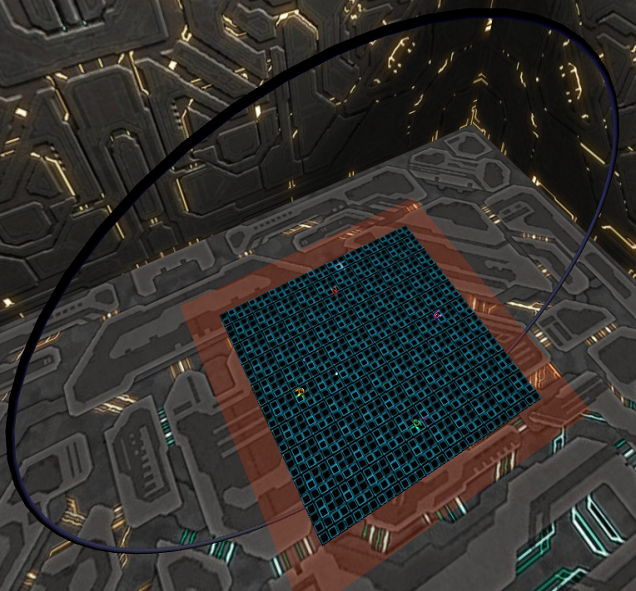
\includegraphics[width=\linewidth]{giorno}
		\caption{Day modality}
	\end{minipage}
	\hfill
	\begin{minipage}[b]{0.45\linewidth}
		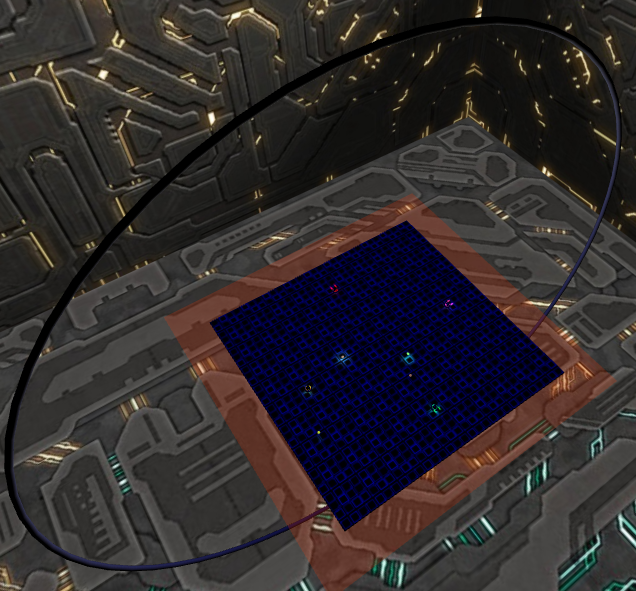
\includegraphics[width=\linewidth]{notte}
		\caption{Night modality}
	\end{minipage}
\end{figure}

The halo object is used to simulate the day-night cycle and it is implemented in the Halo.js file.

We have implemented the halo object with a group, which is composed by a torus and two spotlight, one for the sun and the other for the moon. Those spotlight are positioned in opposite part of the torus and both points to the centre of the game plane. The difference between the lights is the colour of the light.  
In order to simulate the cycle we used a rander function, that will rotate the torus by 0.5 degrees each frame.

The modality of the Halo can be choose in the main menu; we have:
\begin{itemize}
	\item day: the torus starts in the day configuration and won't rotate.
	\item night: the torus starts in the day configuration and won't rotate.
	\item cycle: day: the torus starts in the day configuration and will rotate.
\end{itemize}
The differences between day and night can be seen in the figure above.
\FloatBarrier

\subsection{Animated Light}

An animated Light is a sphere that emits light and move in the space. This is implemented in the animatedLight.js file.

Each light is a point light, and is constructed by generating a set of random points in the space, delimited by the plane space, and a random colour. Then those points are interpolated using a closed loop CatmullRomCurve3, from THREE. Since the position of the light in the curve is defined in the interval from 0 and 1, we increment the position, at each frame, with a small delta, in order to simulate the movement . This is done is the render function.  	
\begin{figure}
	\centering
	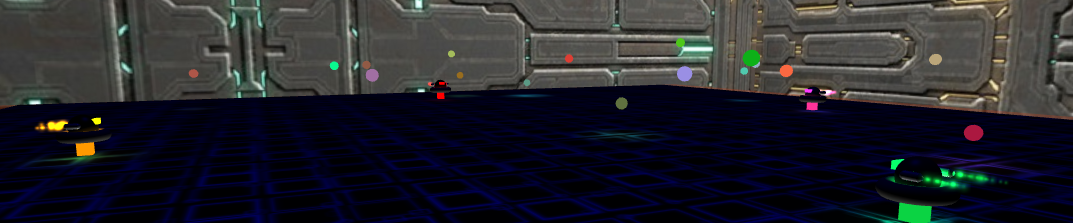
\includegraphics[width=\linewidth]{animatedLight}
	\caption{some animated lights}
\end{figure}
\FloatBarrier

\subsection{Plane and skybox}

\begin{wrapfigure}{r}{0pt}
	\centering
	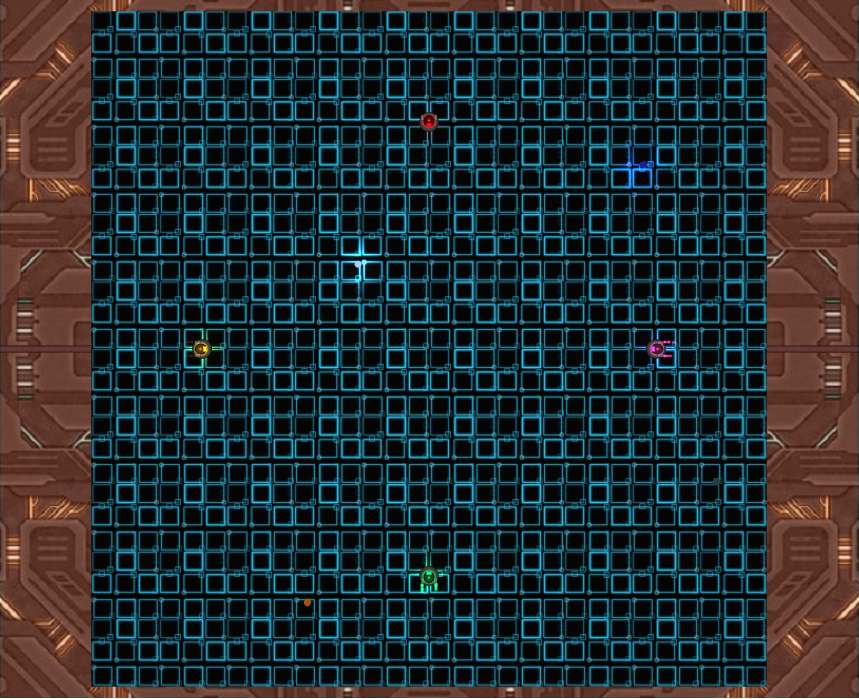
\includegraphics[width=0.4\linewidth]{plane}
	\caption{the plane and the red square}
\end{wrapfigure}
The plane is a transparent square, in which the ships can move; the material is a Phong type. Below the plane we have a red transparent flat square, that indicates the zone in which the ships cannot go. The material of the red square is a basic mash material.

The skybox is simply the composition of two texture, one repeated two time, for the bottom and the top, and another repeated and rotated four time. Those texture composed form the skybox cube.

\newpage
\section{Game Logic and rendering}
In this section we will analyse the game logic, the render part of the game and the animations of the ship. 
\subsection{Main loop and render}

The main loop is the \textit{animate} function. 

If the game is running we check for collisions and see if the game ending conditions are met. Respectively using the \textit{collision} function and the \textit{checkEnd}. The collision logic will be explained later. In the \textit{checkEnd} we also move the players; the movement of the player will be explained in \textit{animations and player movement}.

If the game is on pause we check for every button is pressed, and based on the state of the game we display some menu; the menu section will cover this part. Then, depending on the active scene, the game or the menu, the function will call a different render function. 

In the render of the menu we rotate the ships, update theirs particle motors and modify the colour of each ship, depending on the chosen one, while in the render of the game we move the ships, the animated lights and rotate the halo, if the cycle is selected as modality of the light. Moreover we set the camera to follow the player if the single player mode is selected. 
In the render of the game we also animate the ships; the animation \textit{animations and player movement}.

\subsubsection{Collision}
The collision are implemented using the Box3 class from Three.js.
For each ship we compute te bounding box of the cabin, and for each wall we compute the bounding box of the entire wall segment. 
Each player control contains the box of the cabin and an array with the box of the players walls.
The collision check consist of some basic controls inside some loops.

If the player cross the plane boundary then will die. Elsewhere, for each player, we iterate over all the walls and over all others player's ship box. If the collision test with walls will result positive then the player will die, but if the player collides with another player both will die.
If a player is dead there is no reason to check collision.

\subsection {animations and player movement}
Each ship is animated in the render function, calling the render function in the player.js file. The animation consists in moving the ship on y axis following a sin function and rotating the torus by certain amount of degrees. Moreover all the particles of the motors will be updated.

In this file we check if the player is dead or not. If it is dead then the explosion animation will start. The explosion animation consist on a certain amount of particles (sprites) and an animation of the ship.Each particle will move from the explosion point to a random point in the plane, with a parabolic movement, using CatmullRomCurve3 from \textit{Three.js}. Like in the case of the animated lights, the curve position is defined from 0 to 1. So each frame start at 0 position, and when reach the position 1 will be deleted. In the animation of the ship the motors will continues to go straight ahead, the torus will fall on the ground and the cabin with the glass will rotate and going up. Meanwhile the ship and the will shrink.

When the animation is over the ship and the walls will disappear from the scene.

\begin{figure}
	\centering
	\begin{minipage}[b]{0.8\linewidth}
		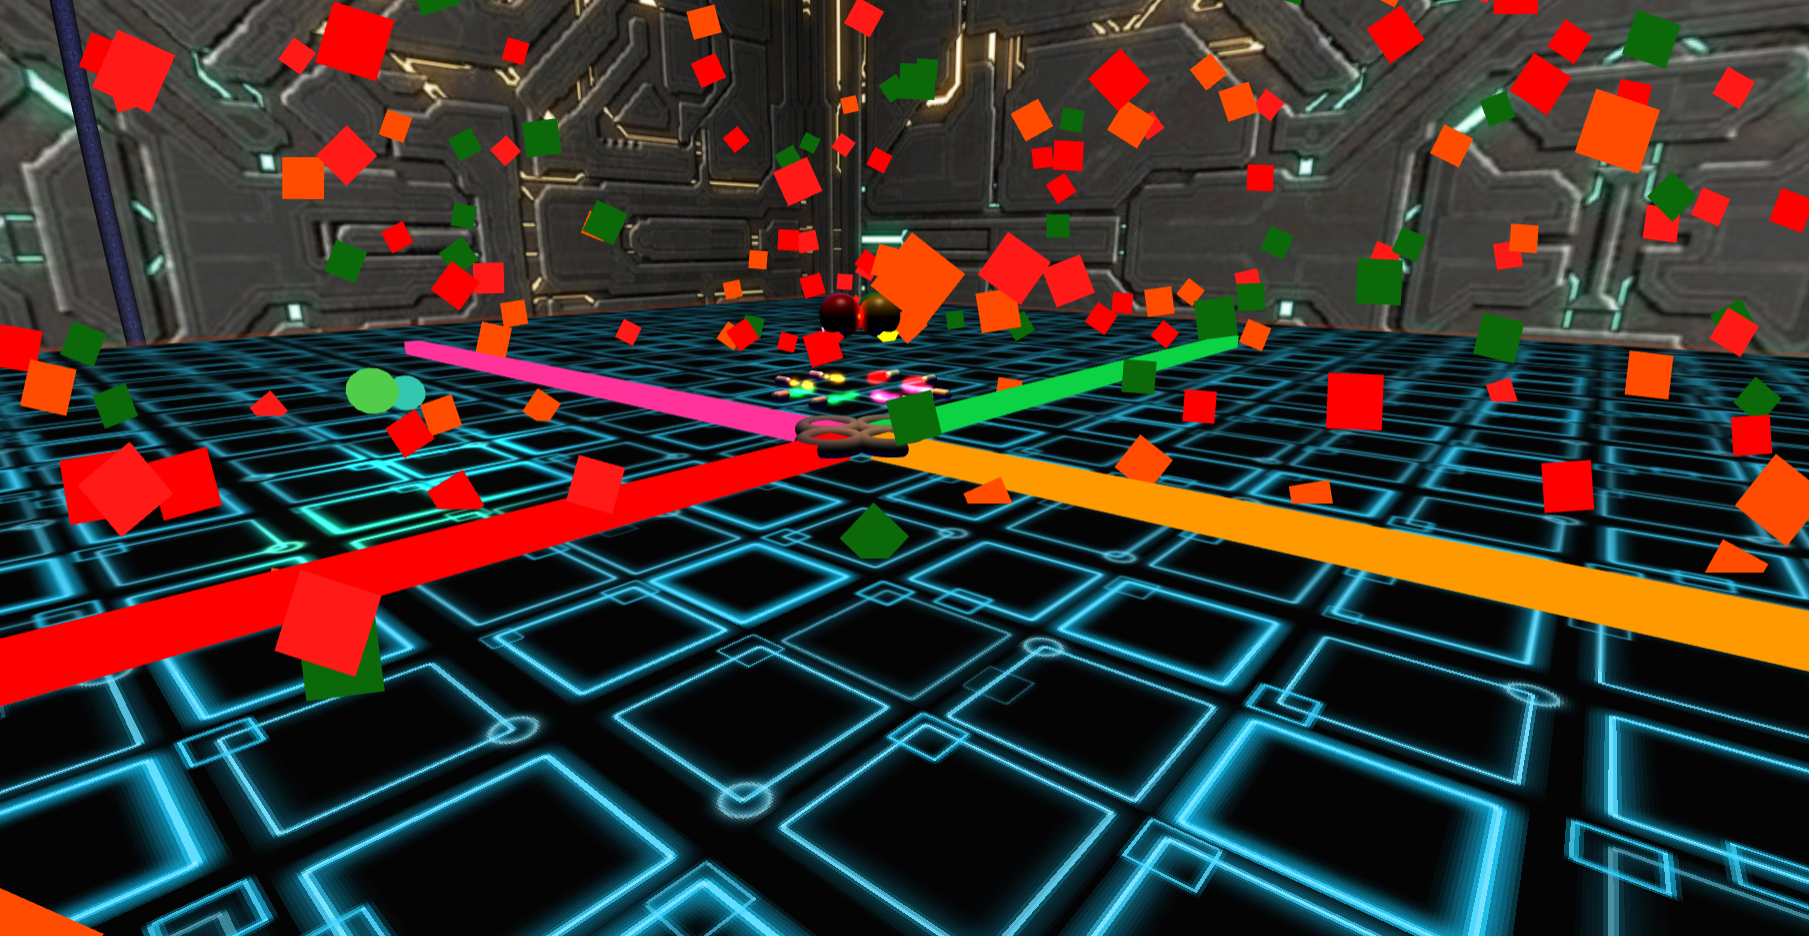
\includegraphics[width=\linewidth]{collision}
		\caption{Collision between 4 ships}
	\end{minipage}
	\hfill
	\begin{minipage}[b]{0.4\linewidth}
		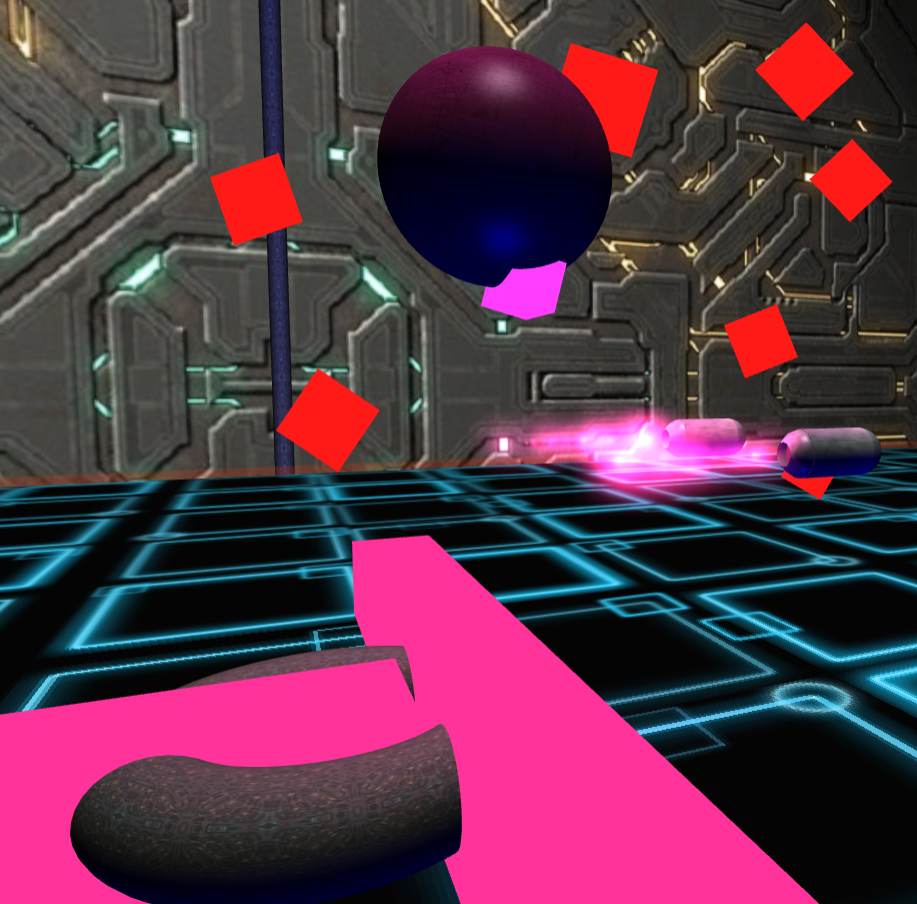
\includegraphics[width=\linewidth]{explosion}
		\caption{Animation of the explosion}
	\end{minipage}
\end{figure}
\FloatBarrier

Since the ships can move only on two coordinates, and rotate  only by 90 degrees, we implemented the movement with a unitary vector of dimension 3, in which only one value is set to 1 or -1, and the other are set to 0. This value indicates the direction of the ship respect to the centre of the plane. 

This vector is used also to generate the walls, from the last point in which the ship turned to the current point.
\subsection{Menu}
\FloatBarrier


	The game contains several menu views: The \textbf{main menu} (fig. 15), \textbf{key settings} (fig. 14), \textbf{colour settings} (fig. 16), \textbf{end game} (fig. 11,12,13), \textbf{pause} (fig. 17).\\
	
	The main menu allow the users to start the game, to go in the key settings menu or to the colour settings menu.
	Furthermore, it allow to change the principal settings of the game: choose the number of playing players, decide if allow the main soundtrack and the in-game sound effect, only the last one or to play without any kind of sounds, and finally to choose between the three light modalities, \textbf{day}, \textbf{night} or \textbf{cycle}.
	
	Next to the main menu, there are a view of all the 4 ships, below there is a pillar representing the ranking position of the relative player (fig. 18).
	Furthermore, the players with the higher score are lit up by a spotlight, except if they are all on the same score.\\
	
	The key settings menu is used in order to modify the default value of the command for each player. In the menu is shown, fore each player, the relative number of the player with the choosen colour and two button, usable to change the \textit{turn-left} and \textit{turn-right} commands values.\\
	
	In the colour setting menu we can find three slider fore each player, relative to the RGB colour, and a bar coloured with the result of the three component.
	
	On the left of this menu are showed the four ships with their chosen relative colours.
	
	When only one player still alive, if the initial number of player was at least 2, the end game menu is showed, in which we find a table showing the ranking of the players in game. In this table there are the numbers relative of each player, if the colour is grey, it means that the relative player is not playing, otherwise are shown the colours relative to the player.
	Furthermore, in the same menu are shown two button, one to come back to main menu, other to play again the game.\\
	
	Finally there is a pause menu, where we can find three buttons: the same two button described in the end game menu and another one to show the key settings menu.
	
	 \begin{figure}
	 	\centering
	 	\begin{minipage}[b]{0.25\linewidth}
	 		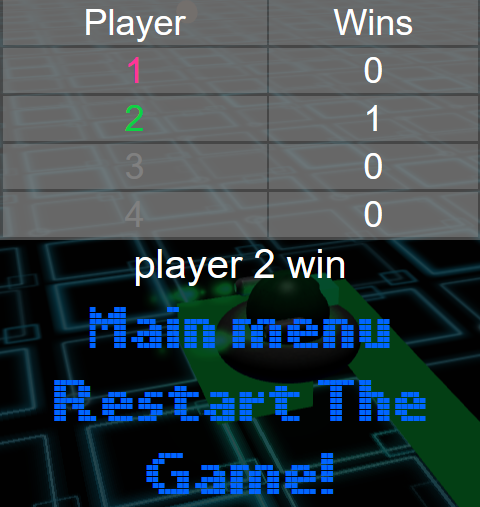
\includegraphics[width=\linewidth]{endGameMenu2}
	 		\caption{with 2 player}
	 		\label{fig:endGameMenu2}
	 	\end{minipage}
	 	\begin{minipage}[b]{0.25\linewidth}
	 		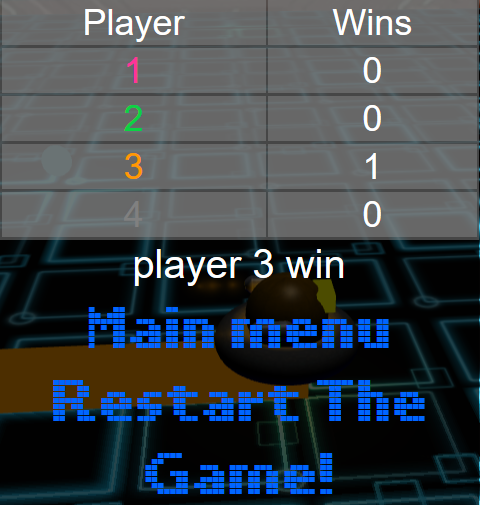
\includegraphics[width=\linewidth]{endGameMenu3}
	 		\caption{with 3 player}
	 		\label{fig:endGameMenu3}
	 	\end{minipage}
	 	\begin{minipage}[b]{0.25\linewidth}
	 		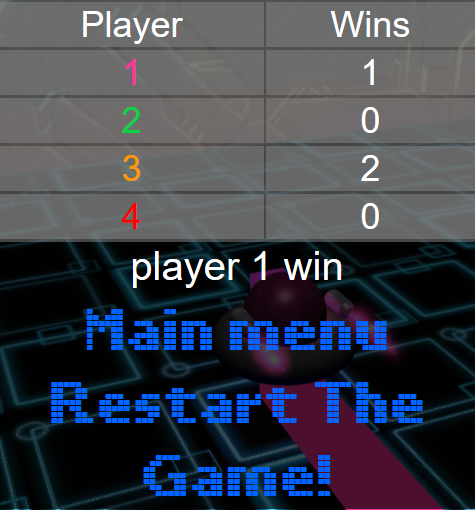
\includegraphics[width=\linewidth]{endGameMenu4}
	 		\caption{with 4 player}
	 		\label{fig:endGameMenu4}
	 	\end{minipage}
	 \end{figure}
	 

\begin{figure}
	\centering
	\begin{minipage}[b]{0.25\linewidth}
		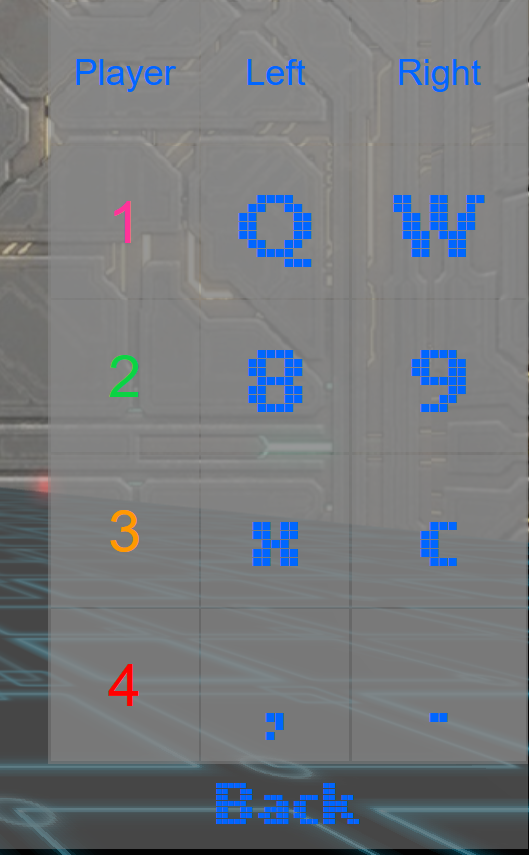
\includegraphics[width=\linewidth]{keySettingsMenu}
		\caption{This is the menu used to change the default controls value.}
		\label{fig:keySett}
	\end{minipage}
	\begin{minipage}[b]{0.25\linewidth}
		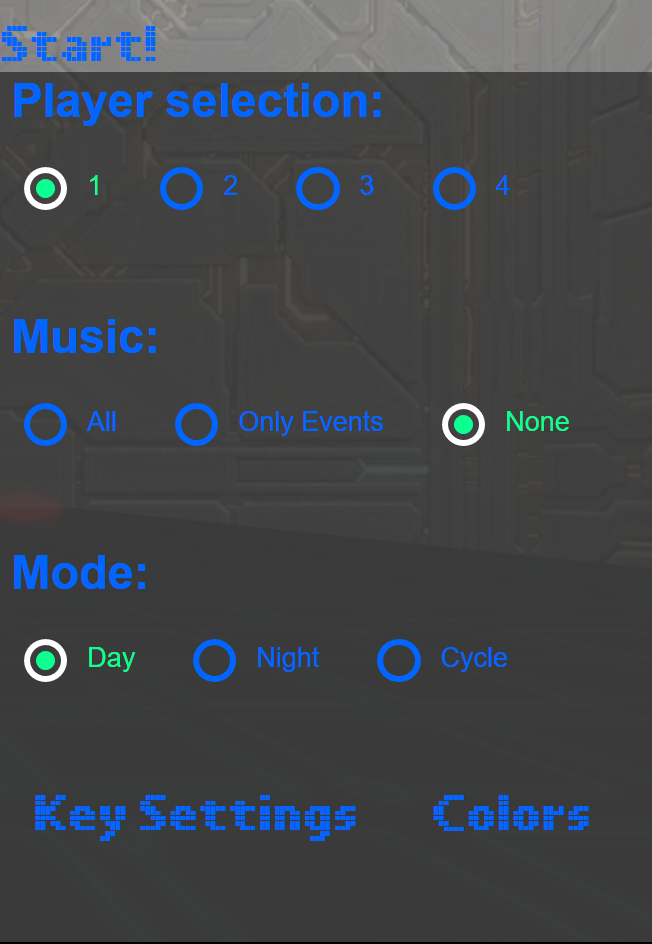
\includegraphics[width=\linewidth]{startMenu}
		\caption{This is the main menu, used to start the game or to change some of the principal settings.}
		\label{fig:startMenu}
	\end{minipage}
\hfill
	\begin{minipage}[b]{0.6\linewidth}
		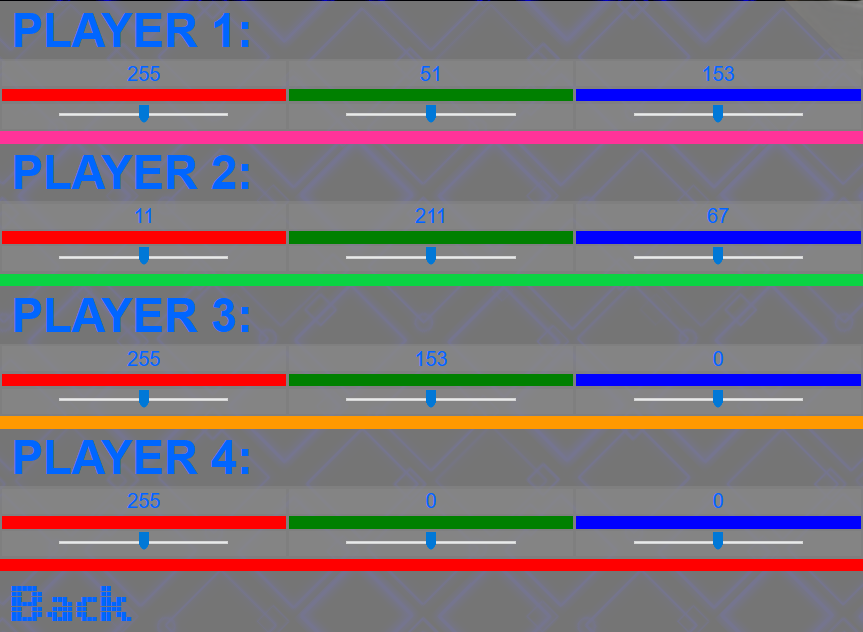
\includegraphics[width=\linewidth]{colorMenu}
		\caption{This is the menu used to change the default colours value.}
		\label{fig:colorMenu}
	\end{minipage}
	\begin{minipage}[b]{0.4\linewidth}
		
\includegraphics[width=\linewidth]{pauseMenu}
		\caption{This is the pause menu}
		\label{fig:endGameMenu4}
	\end{minipage}
	\begin{minipage}[b]{0.6\linewidth}
		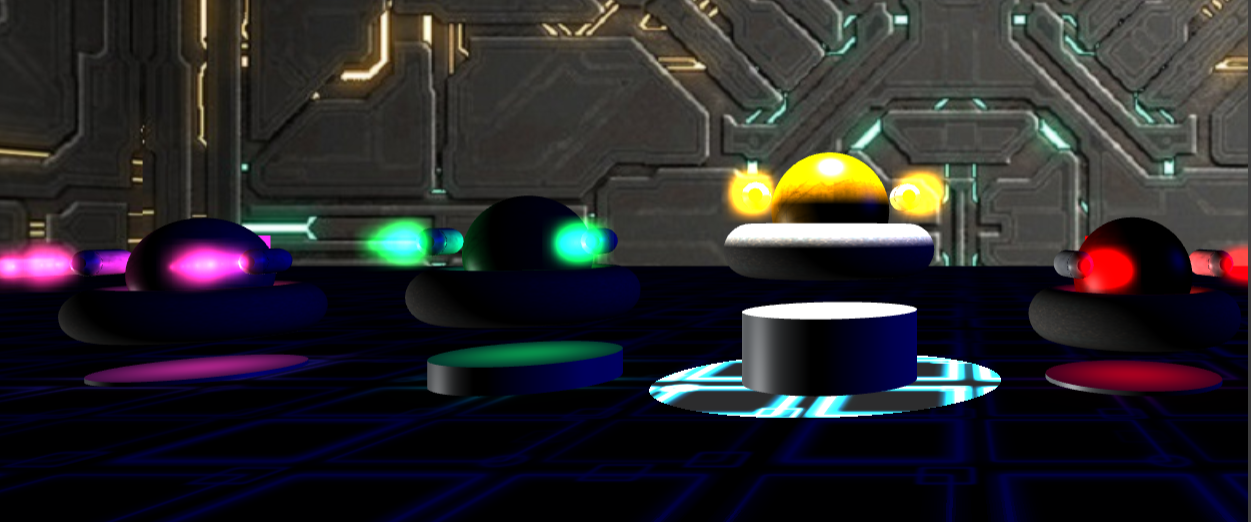
\includegraphics[width=\linewidth]{Ranking}
		\caption{This is the ranking shown in the main menu.}
		\label{fig:Ranking}
	\end{minipage}
\end{figure}

\end{document}
